
\usetikzlibrary{arrows}
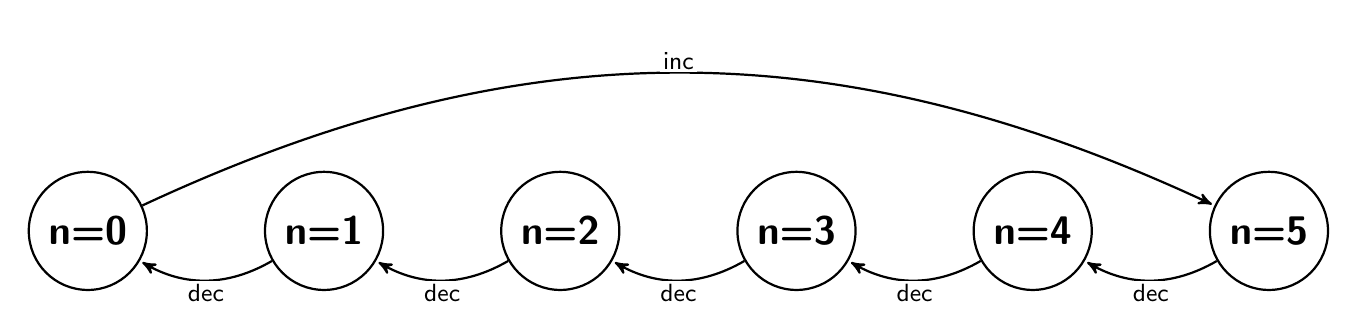
\begin{tikzpicture}[->,>=stealth',shorten >=1pt,auto,node distance=3cm,
  thick,main node/.style={circle,fill=white!20,draw,
  font=\sffamily\Large\bfseries,minimum size=15mm}]

  \node[main node] (A) {n=0};
  \node[main node] (B) [right of=A] {n=1};
  \node[main node] (C) [right of=B] {n=2};
  \node[main node] (D) [right of=C] {n=3};
  \node[main node] (E) [right of=D] {n=4};
  \node[main node] (F) [right of=E] {n=5};

  \path[every node/.style={font=\sffamily\small,
  		fill=white,inner sep=1pt}]
  	% Right-hand-side arrows rendered from top to bottom to
  	% achieve proper rendering of labels over arrows.
    (A) edge [bend left=25] node {inc} (F)
    (B) edge [bend left=30] node {dec} (A)
    (C) edge [bend left=30] node {dec} (B)
    (D) edge [bend left=30] node {dec} (C)
    (E) edge [bend left=30] node {dec} (D)
    (F) edge [bend left=30] node {dec} (E);
   
\end{tikzpicture}
\\